% ==============================================================================
% sci_s1_overview.tex — SCI/SICE tutorial Session 1:
% overview and design philosophy of StampFly Ecosystem
% SCI/SICE チュートリアル セッション1: StampFly Ecosystem の全体像と設計思想
% ==============================================================================

% ------------------------------------------------------------------
\begin{frame}{開発サイクルの地図と今の位置（セッション1）}
  \begin{columns}[c]
    \begin{column}{0.5\textwidth}
      \centering
      \resizebox{\columnwidth}{!}{\scisessionmap{1}}
    \end{column}
    \begin{column}{0.47\textwidth}
      \small
      今日はこの循環を 5 つのセッションで 1 周する。まずは全体像と設計思想から
    \end{column}
  \end{columns}
\end{frame}

% ------------------------------------------------------------------
\begin{frame}{StampFly Ecosystem とは何か: 目的・考え方・提供物}
  \begin{enumerate}
    \item \textbf{何のために}: 制御なしには飛べないマルチコプタを教材にし、一人の学習者が 1 機で「設計 $\to$ 実装 $\to$ 実験 $\to$ 解析」を自分の手で一周できるようにする
    \item \textbf{どういう考え方で}: 一つのリポジトリ・4 階層の入口・同じコードとモデルで実機とシミュレータをつなぐ（5 つの設計の考え方）
    \item \textbf{何を提供するか}: 機体、ファームウェア、3 種類のシミュレータ、sf CLI、そして 8 分野を通る教材。本日の実習 1〜9 はその教材の一部
  \end{enumerate}
\end{frame}

% ------------------------------------------------------------------
\begin{frame}{目的: 制御がなければ飛べない}
  \vspace{0.3em}

  \small マルチコプタは固定翼機のように滑空できず、ヘリコプタのようにオートローテーションで降りることもできない。制御系が止まれば即座に墜落する

  \vspace{0.5em}

  \begin{exampleblock}{教材としての魅力}
    \small この性質は安全上の課題であると同時に、学習者が「制御がなければ飛べない」という事実を身をもって体験できる特性でもある。フィードバック制御の役割を直感的に理解する入口になる
  \end{exampleblock}
\end{frame}

% ------------------------------------------------------------------
\begin{frame}{目的: 教材として使うには 4 つの障壁がある}
  \small 制御なしには飛べないマルチコプタは制御教育の教材として魅力的だが、実際の教育現場で使うには次の 4 つの障壁がある

  \vspace{0.5em}

  \begin{itemize}\small\setlength{\itemsep}{4pt}
    \item \textbf{ブラックボックス問題}: 市販の教育用ドローンは飛ぶが、制御ループの中身に触れられない
    \item \textbf{理論と実装のギャップ}: PIDの数式は教科書で学べても、組込みのリアルタイム制御ループとして実装するには別のスキルが要る
    \item \textbf{体系的教材の不在}: センサ取得から状態推定、制御、実験、データ解析までを一貫して学べる教材が見当たらない
    \item \textbf{教育者の準備負担}: カリキュラム設計・教材作成・ツール整備を一人の教育者がすべて担うのは現実的でない
  \end{itemize}
\end{frame}

% ------------------------------------------------------------------
\begin{frame}{目的: 既存プラットフォームとの比較}
  {\small 既存のプラットフォームは、この 4 つの障壁のどれかが残る}
  \begin{table}
    \centering\footnotesize
    \begin{tabular}{lcccc}
      \hline
       & Crazyflie & Tello EDU\textsuperscript{*} & PX4 & StampFly Eco. \\
      \hline
      制御ループアクセス & \checkmark & --- & \checkmark & \checkmark \\
      教材・カリキュラム & $\triangle$ & $\triangle$ & $\triangle$ & \checkmark \\
      シミュレータ統合   & \checkmark & --- & \checkmark & \checkmark \\
      コスト             & 高 & 低 & 高 & 低 \\
      コード規模         & 中 & --- & 大 & 小 \\
      \hline
    \end{tabular}
  \end{table}

  \vspace{0.5em}

  {\small 制御ループへのフルアクセスと体系的な教材・ツールの統合提供を両立させ、ファームウェア全体を一人の学習者が読み通せる規模に抑えている点が異なる}

  {\scriptsize \textsuperscript{*}Tello EDU は2023年末に販売終了（評価は筆者の定性的見解）}
\end{frame}

% ------------------------------------------------------------------
\begin{frame}{目的: StampFly Ecosystem が目指すもの}
  \begin{block}{一人の学習者が、1 機の機体で、制御設計の循環を自分の手で一周できるようにする}
    \footnotesize 設計（モデルとゲイン）$\to$ 実装（コード）$\to$ 実験（実機と SILS）$\to$ 解析（ログの可視化と同定）$\to$ 次の設計へ。対象は制御を学ぶ学生・研究者と教育者
  \end{block}

  \begin{table}
    \centering\scriptsize
    \renewcommand{\arraystretch}{1.1}
    \begin{tabular}{lp{92mm}}
      \hline
      \textbf{障壁} & \textbf{Ecosystem の答え} \\
      \hline
      ブラックボックス問題 & 制御ループからドライバまで全部を公開し、学習者が読み通せる規模に抑える \\
      理論と実装のギャップ & 実機と同じコードをシミュレータでも動かし、数式と組込み実装を切れ目なく扱う \\
      体系的教材の不在 & センサ取得・状態推定・制御・実験・解析を 1 機で通る教材とツールを同梱する \\
      教育者の準備負担 & 教材・実習コード・ビルドと書き込みの道具を一式で配り、準備を減らす \\
      \hline
    \end{tabular}
  \end{table}
\end{frame}

% ------------------------------------------------------------------
\begin{frame}{思想: 5 つの Ecosystem 設計の考え方}
  \begin{table}
    \centering\footnotesize
    \renewcommand{\arraystretch}{1.2}
    \setlength{\tabcolsep}{8pt}
    \begin{tabular}{lp{104mm}}
      \hline
      \textbf{考え方} & \textbf{内容} \\
      \hline
      一つのリポジトリ & ファーム・シミュレータ・解析ツール・教材を一か所にまとめる。通信仕様の定義は一つだけ置き、各実装はそこから作る \\
      sf CLI & ビルド・書込み・ログ取得・シミュレーションを一つのコマンド体系で操作する \\
      4 階層アクセス & 実習用 API からハードウェアの直接操作まで 4 つの入口を用意し、必要な深さから入る \\
      シミュレータ統合 & 軽量 3D（VPython）・高精度物理（Genesis）・実ファーム実行（SILS）の 3 つを使い分け、同じ物理パラメータとゲインでつなぐ \\
      オープンソース & 制御ループからドライバまで全部を公開し、ブラックボックスを作らない \\
      \hline
    \end{tabular}
  \end{table}
\end{frame}

% ------------------------------------------------------------------
\begin{frame}{思想: 4 階層アクセス（必要な深さから入る）}
  \centering
  \vspace{-1mm}
  \resizebox{!}{0.82\textheight}{% sci_tier_access.tex — 4-tier learner-entry-point diagram for the SCI tutorial
% 4階層アクセス（学習者の入口）図。SCIチュートリアル用。
%
% Source of the four tiers: firmware/vehicle/docs/architecture.md §2
% 「学習者の入口（4階層アクセス）」の表を図として再構成したもの。
%
% Layout: four stacked boxes, top = highest abstraction (L0, beginners),
% bottom = lowest abstraction (L3, firmware implementers). A downward arrow
% chain to the right of the boxes shows that a learner may step down as far
% as their topic requires; each tier is otherwise usable on its own.
% レイアウト: 4段の箱を縦に積む。上ほど抽象度が高く（L0・初心者向け）、
% 下ほど抽象度が低い（L3・ファーム実装者向け）。箱の右側の下向き矢印は、
% 学習者が必要な分だけ下の層へ降りられることを示す（各層は単独でも使える）。
\documentclass[border=10pt]{standalone}
\usepackage{tikz}
\usetikzlibrary{arrows.meta, positioning, calc}
\usepackage{luatexja}
\usepackage[match]{luatexja-fontspec}
% Cross-platform font: Hiragino (macOS) → Yu Gothic (Windows) → Noto (Linux)
% クロスプラットフォーム: ヒラギノ (macOS) → 游ゴシック (Windows) → Noto (Linux)
\usepackage{ifthen}
\newboolean{jfontset}\setboolean{jfontset}{false}
\IfFontExistsTF{Hiragino Kaku Gothic ProN}{%
  \setmainjfont{Hiragino Kaku Gothic ProN}%
  \setsansjfont{Hiragino Kaku Gothic ProN}%
  \setboolean{jfontset}{true}}{}
\ifthenelse{\boolean{jfontset}}{}{%
  \IfFontExistsTF{Yu Gothic}{%
    \setmainjfont{Yu Gothic}%
    \setsansjfont{Yu Gothic}%
    \setboolean{jfontset}{true}}{}}
\ifthenelse{\boolean{jfontset}}{}{%
  \IfFontExistsTF{Noto Sans CJK JP}{%
    \setmainjfont{Noto Sans CJK JP}%
    \setsansjfont{Noto Sans CJK JP}}{}}

\begin{document}

\definecolor{l0color}{RGB}{0, 100, 180}
\definecolor{l1color}{RGB}{40, 140, 60}
\definecolor{l2color}{RGB}{120, 80, 150}
\definecolor{l3color}{RGB}{110, 110, 110}
\definecolor{gray1}{RGB}{120, 120, 120}

% Plain-LaTeX helper macros for the colored text lines inside each box
% (kept as ordinary commands, not tikz styles, since they are used inside
% node text rather than as tikzpicture options)
% 箱の中の色付きテキスト用マクロ（ノードのテキスト内で使うのでtikzの
% オプションではなく普通のLaTeXコマンドとして定義する）
\newcommand{\ttier}[2]{{\bfseries\large\color{#1}#2}}
\newcommand{\tns}[2]{{\ttfamily\normalsize\color{#1}#2}}
\newcommand{\tsub}[1]{{\small\color{black!55}#1}}

\begin{tikzpicture}[
    tier/.style={
      rectangle, rounded corners=4pt, draw=#1, line width=1.5pt,
      fill=#1!8, minimum width=92mm, minimum height=25mm,
      align=left, inner xsep=10mm, inner ysep=2mm
    },
    arr/.style={-{Stealth[length=3.2mm]}, line width=1.6pt, gray1},
  ]

  % Four tiers, top (L0, most abstract) to bottom (L3, closest to hardware)
  % 4層。上（L0・最も抽象的）から下（L3・ハードウェアに最も近い）まで
  \node[tier=l0color] (L0) at (0, 0) {%
    \begin{minipage}{86mm}\raggedright
      \ttier{l0color}{L0: Workshop API}\quad\tns{l0color}{ws::*}\\[3pt]
      \tsub{典型ユーザー: Workshop 受講者}\\[1pt]
      \tsub{setup() / loop\_400Hz(dt)、30+ 関数で完結}
    \end{minipage}%
  };
  \node[tier=l1color, below=12mm of L0] (L1) {%
    \begin{minipage}{86mm}\raggedright
      \ttier{l1color}{L1: Topic API}\quad\tns{l1color}{sf::api::*}\\[3pt]
      \tsub{典型ユーザー: 推定・制御学習者}\\[1pt]
      \tsub{Topic を subscribe/publish、IEstimator/IController 差替え}
    \end{minipage}%
  };
  \node[tier=l2color, below=12mm of L1] (L2) {%
    \begin{minipage}{86mm}\raggedright
      \ttier{l2color}{L2: HAL Direct}\quad\tns{l2color}{stampfly::*Wrapper}\\[3pt]
      \tsub{典型ユーザー: HW 学習者}\\[1pt]
      \tsub{SPI / I2C を直接呼ぶ（Topic を介さない経路）}
    \end{minipage}%
  };
  \node[tier=l3color, below=12mm of L2] (L3) {%
    \begin{minipage}{86mm}\raggedright
      \ttier{l3color}{L3: BSP Internal}\quad\tns{l3color}{sf::internal::board}\\[3pt]
      \tsub{典型ユーザー: ファーム実装者}\\[1pt]
      \tsub{bus handle、起動順序を直接扱う}
    \end{minipage}%
  };

  % Downward arrow chain, connecting each box directly at its center
  % (Lk.south -> L(k+1).north), so the arrowhead touches the box below.
  % Fix: the previous version drew the arrows 10mm to the right of the
  % boxes, floating in open space and touching nothing (T3 violation).
  % 下向き矢印の連鎖。各箱を中心で直結する（Lk.south -> L(k+1).north）。
  % 矢頭が下の箱に接する。修正: 以前は箱の右10mmにオフセットして描画
  % しており、何にも接続しない宙に浮いた矢印だった（T3違反）。
  \draw[arr] (L0.south) -- (L1.north);
  \draw[arr] (L1.south) -- (L2.north);
  \draw[arr] (L2.south) -- (L3.north);

  % Single side label for the whole arrow chain (vertically centered)
  % 矢印の連鎖全体に対する説明ラベル（縦方向の中央に1つだけ配置）
  \coordinate (midy) at ($(L1.south)!0.5!(L2.north)$);
  \node[rotate=270, font=\small, text=gray1, align=center,
        anchor=center] at ($(midy -| L0.east) + (26mm, 0)$)
    {必要な分だけ降りられる\\（各層は単独でも使える）};

\end{tikzpicture}
\end{document}
}
\end{frame}

% ------------------------------------------------------------------
\begin{frame}{思想: 実機とシミュレータをつなぐ 3 原則}
  \begin{table}
    \centering\footnotesize
    \begin{tabular}{lp{100mm}}
      \hline
      \textbf{原則} & \textbf{内容} \\
      \hline
      Code Identity  & \textbf{同じコードで動く。}SILS は実機と同じファームウェアのソースをそのまま組み込んで動かす。推定や制御の式だけでなく、制御ループ全体が実機と同一 \\
      Parameter Identity & \textbf{同じ設定値で動く。}ゲインなどの調整値は SILS と実機が同じ一覧から読む。片方で決めた値をそのまま他方へ持ち込める \\
      Model Fidelity & \textbf{正解は物理モデルから作る。}SILS の「真値」は物理モデルで作る。実機データが要るのは、初飛行のあとでモデルを現実に近づけるときだけ \\
      \hline
    \end{tabular}
  \end{table}
\end{frame}

% ------------------------------------------------------------------
\begin{frame}{提供: エコシステムの地図}
  \centering
  \vspace{1mm}
  \resizebox{!}{0.78\textheight}{\input{../../_shared/tikz/ecosystem_layers}}
\end{frame}

% ------------------------------------------------------------------
\begin{frame}{提供: 機体 StampFly}
  \begin{columns}[T]
    \begin{column}{0.42\textwidth}
      \centering
      
\includegraphics[width=\columnwidth]{Stampfly_onhand.jpg}
    \end{column}
    \begin{column}{0.56\textwidth}
      \begin{table}
        \centering\footnotesize
        \renewcommand{\arraystretch}{0.82}
        \setlength{\tabcolsep}{3pt}
        \begin{tabular}{lp{58mm}}
          \hline
          \textbf{項目} & \textbf{仕様} \\
          \hline
          MCU        & ESP32-S3（M5StampS3） \\
          IMU        & BMI270（6軸 400\,Hz） \\
          気圧       & BMP280 \\
          磁力計     & BMM150（3軸） \\
          測距       & VL53L3CX $\times$2（Bottom / Front） \\
          光学フロー & PMW3901 \\
          電流電圧   & INA3221 \\
          モータ     & コアレスモータ $\times$4 \\
          バッテリ   & 300\,mAh 1S LiPo \\
          質量       & 37\,g（バッテリ含む） \\
          コントローラ & M5Stack AtomS3 + Atom JoyStick（ESP-NOW） \\
          \hline
        \end{tabular}
      \end{table}
      \vspace{-2pt}

      {\scriptsize IMU（慣性計測装置）／ESP-NOW（ESP32 の無線プロトコル）。前方 ToF は未使用（高度推定は下方 ToF）}
    \end{column}
  \end{columns}
\end{frame}

% ------------------------------------------------------------------
\begin{frame}{提供: 機体ファームウェア（vehicle）}
  \begin{table}
    \centering\footnotesize
    \begin{tabular}{ll}
      \hline
      コンポーネント数 & 30（\code{sf\_*} 命名, フラット構造） \\
      通信方式         & Pub-Sub トピック（直接呼び出し禁止） \\
      タスク数         & 16 \\
      制御周期         & 400\,Hz（IMU $\to$ 状態推定 $\to$ 制御） \\
      状態推定         & ESKF（誤差状態カルマンフィルタ） \\
      制御器           & カスケード PID \\
      飛行モード       & ACRO / STABILIZE / ALT\_HOLD / POS\_HOLD \\
      \hline
    \end{tabular}
  \end{table}

  {\footnotesize Pub-Sub（出版購読型のメッセージ配信）}

  \vspace{0.3em}

  \begin{exampleblock}{実機検証}
    \small POS\_HOLD（位置制御）は実機で検証済み。保持精度 $\pm$6--7\,cm
  \end{exampleblock}
\end{frame}

% ------------------------------------------------------------------
\begin{frame}{提供: 400\,Hz 制御ループ}
  \centering
  \vspace{-1mm}
  \resizebox{0.82\textwidth}{!}{\input{../../_shared/tikz/loop_400hz_timeline}}

  \vspace{0.3em}

  {\small IMU 割込みを起点に、状態推定 $\to$ 制御 $\to$ アクチュエーションが 2.5\,ms 周期で走る。全コンポーネントが同じ周期を共有する}
\end{frame}

% ------------------------------------------------------------------
\begin{frame}{提供: シミュレータ --- 役割の違う 3 つの実行環境}
  \begin{table}
    \centering\scriptsize
    \renewcommand{\arraystretch}{1.2}
    \setlength{\tabcolsep}{4pt}
    \begin{tabular}{p{15mm}p{40mm}p{28mm}p{24mm}p{22mm}}
      \hline
      \textbf{名前} & \textbf{役割} & \textbf{物理モデル} & \textbf{動く制御コード} & \textbf{可視化} \\
      \hline
      SILS & \textbf{ファームの開発と制御系の実装を、机上である程度完了させる}。飛ばす前の検証と合否判定（実習 8 (2/2)） & MuJoCo（外部エンジン、物理計算のみ）＋自作のモータ・センサ・風モデル & 実機と同じ C++ ファームそのもの & ブラウザ GUI（three.js の 3D とグラフ） \\
      VPython 版 & \textbf{練習用}。簡単で読みやすい Python で、力学エンジン・3D 表示・センサモデルなど「シミュレータの作り方」を学ぶ（デモ①） & 自作の 6 自由度モデル & Python に移植した制御則 & VPython のブラウザ 3D \\
      Genesis 版 & \textbf{強化学習向けの選択肢}として残している。今日は使わない & Genesis（外部の高精度エンジン） & Python の制御則 & Genesis の 3D \\
      \hline
    \end{tabular}
  \end{table}

  \begin{block}{なぜ 1 つでは足りないか}
    \footnotesize 「実機のファームをそのまま動かして検証する」「中身を読んで作り方を学ぶ」「強化学習を回す」は要求が違い、1 つの実装では両立しない。3 つは同じ物理パラメータ（\code{stampfly\_physical.yaml}、\code{sf params check} で照合）を共有する
  \end{block}
\end{frame}

% ------------------------------------------------------------------
\begin{frame}{提供: SILS の仕組み --- 実機のファームを PC で走らせる}
  \begin{columns}[T]
    \begin{column}{0.52\textwidth}
      \begin{itemize}\scriptsize\setlength{\itemsep}{1pt}
        \item \textbf{ファームは無改変}: 実機に書き込む vehicle のソースをそのまま PC 向けにコンパイル（状態機械・フェイルセーフも含む）
        \item \textbf{OS の代わり}: 仮想時計で動く決定論的な疑似 RTOS と ESP-IDF 互換スタブ。同じ入力なら毎回同じ結果
        \item \textbf{制御対象}: MuJoCo（6 自由度）＋自作のモータ・センサ・風モデル。400\,Hz でファームと歩調を合わせる
        \item \textbf{試験の与え方}: シナリオ \code{.scn} に操縦・外乱・故障を時系列で書き、\code{.expect} で PASS / FAIL を自動判定。CI で既存動作の破壊を検出
        \item \textbf{実習コードも同じ土俵}: 参加者の \code{user\_code.cpp} も同じ仕組みで飛ぶ（実習 8 (2/2)）
        \item できないこと: 複数タスクの競合、実際の WiFi / ESP-NOW の電波
      \end{itemize}
    \end{column}
    \begin{column}{0.46\textwidth}
      \centering
      \begin{tikzpicture}[
        box/.style={draw, rounded corners=1pt, align=center, font=\scriptsize, minimum width=44mm, inner sep=3pt},
        arr/.style={-{Latex[length=1.5mm,width=1.2mm]}, line width=0.5pt},
        node distance=3.5mm and 0mm]
        \node[box, fill=sfblue!8] (scn) {シナリオ \code{.scn}\\操縦入力・外乱・故障の時系列};
        \node[box, fill=sfblue!15, below=of scn, minimum height=10mm] (fw) {実機と同じファームウェア C++\\（疑似 RTOS ＋ 互換スタブの上）};
        \node[box, fill=sfblue!8, below=of fw, minimum height=10mm] (plant) {制御対象: MuJoCo 6 自由度\\＋ モータ・センサ・風モデル};
        \node[box, fill=sfblue!8, below=of plant] (chk) {ログ ＋ \code{.expect} で合否判定};
        \draw[arr] (scn.south) -- (fw.north);
        \draw[arr] ([xshift=-12mm]fw.south) -- ([xshift=-12mm]plant.north);
        \node[font=\tiny, anchor=east] at ([xshift=-13mm, yshift=-2.5mm]fw.south) {モータ指令};
        \draw[arr] ([xshift=12mm]plant.north) -- ([xshift=12mm]fw.south);
        \node[font=\tiny, anchor=west] at ([xshift=13mm, yshift=-2.5mm]fw.south) {センサ値};
        \draw[arr] (plant.south) -- (chk.north);
      \end{tikzpicture}
    \end{column}
  \end{columns}
\end{frame}


% ------------------------------------------------------------------
% sf sils gui is listed in this session's review path, so show it once here
% (what the screen looks like). How to use it and the hands-on are in S5.
% 復習パスに sf sils gui が載るので、ここで 1 枚だけ画面を見せる。
% 使い方と実習は S5 で扱う。
\begin{frame}[fragile]{提供: SILS を画面で触る（sf sils gui）}
  \vspace{0.15em}

  \begin{columns}[T]
    \begin{column}{0.58\textwidth}
      \centering
      % Screenshot: pos_roll scenario just after a run (headless Chromium capture)
      % 画面写真: pos_roll シナリオ実行直後（ヘッドレス Chromium で撮影）
      \includegraphics[width=\columnwidth]{sils_gui.png}\\[0.2em]
      {\scriptsize \code{pos\_roll} シナリオ実行直後。左: イベント列、右上: 3D 再生、右下: グラフ（時刻カーソルが 3D と同期）、右上端: 合否 12/12 PASS}
    \end{column}
    \begin{column}{0.40\textwidth}
      \begin{itemize}\footnotesize\setlength{\itemsep}{1pt}
        \item ブラウザだけで完結: シナリオ作成（外乱・故障などのイベントを表で組む）$\to$ 実行 $\to$ グラフ $\to$ 合否判定
        \item PID ゲイン等 54 項目を画面で編集。再ビルド不要（Parameter Identity）
        \item 使い方と実習はセッション5。今日は画面を覚えるだけでよい
      \end{itemize}

      \vspace{0.2em}

      \begin{sflisting}[basicstyle=\ttfamily\scriptsize]{起動}
sf sils build
sf sils gui
      \end{sflisting}
    \end{column}
  \end{columns}
\end{frame}

% ------------------------------------------------------------------
\begin{frame}{提供: 教材 --- 1 機から学べる 8 分野}
  {\small 教材は 1 機から次の 8 分野を扱う。本日の実習 1〜9 は制御理論・センサ工学・アクチュエータ・システム同定・状態推定を通る}

  \vspace{0.15em}

  \begin{table}
    \centering\footnotesize
    \renewcommand{\arraystretch}{1.0}
    \setlength{\tabcolsep}{10pt}
    \begin{tabular}{ll}
      \hline
      \textbf{分野} & \textbf{主な学習項目} \\
      \hline
      制御理論       & PID, カスケード制御, FF/FB, アンチワインドアップ \\
      飛行力学       & 6DoF運動方程式, ホバー条件, NED/Body座標変換 \\
      センサ工学     & IMU, 気圧, 光学フロー, Allan分散, ノイズ解析 \\
      状態推定       & 相補フィルタ, ESKF, センサフュージョン \\
      アクチュエータ & PWM制御, 推力モデル, プロペラ空力特性, ミキサ行列 \\
      システム同定   & 周波数応答, パラメータ推定, モデル検証 \\
      通信・IoT      & ESP-NOW, WiFiテレメトリ, プロトコル設計 \\
      ソフトウェア工学 & リアルタイムタスク, 組込み開発, OSS開発 \\
      \hline
    \end{tabular}
  \end{table}

  \vspace{0.15em}

  {\small これらは独立した知識ではなく、1台の機体の中で密接に関連し合っている。PIDゲインの設計には慣性モーメントやモータ応答特性の知識が要り、推定精度はセンサのノイズ特性に左右される}
\end{frame}

% ------------------------------------------------------------------
\begin{frame}[fragile]{デモ①: シミュレータ操縦}
  \vspace{0.15em}

  {\small \textcolor{sfblue}{\textbf{見るだけ}} ｜ 一緒に打つ ｜ 帰宅後に再現}

  \vspace{0.2em}

  \begin{columns}[T]
    \begin{column}{0.54\textwidth}
      \begin{block}{何を見るか}
        \begin{itemize}\footnotesize\setlength{\itemsep}{0pt}
          \item \code{sf sim run vpython} を手元でも起動
          \item VPythonシミュレータが起動し、実機と同じ制御アルゴリズムが動く
          \item HIDジョイスティック（Atom JoyStick）でそのまま操縦できる
          \item 実機がなくても制御コードの挙動を3Dで確認できる
        \end{itemize}
      \end{block}
    \end{column}
    \begin{column}{0.44\textwidth}
      \centering
      % VPython simulator screenshot (VOXEL terrain, in flight); shared with the DXH deck
      % VPython シミュレータの画面（ボクセル地形・飛行中）。DXH 資料と共用
      
\includegraphics[width=\columnwidth]{simulator_demo.png}\\[0.2em]
      {\scriptsize VPython シミュレータの画面（ボクセル地形を飛行中）}
    \end{column}
  \end{columns}
\end{frame}

% ------------------------------------------------------------------
\begin{frame}{デモ②: 実機 POS\_HOLD 飛行}
  \vspace{0.3em}

  {\small \textcolor{sfblue}{\textbf{見るだけ}} ｜ 一緒に打つ ｜ 帰宅後に再現}

  \vspace{0.5em}

  \begin{block}{何を見るか}
    \begin{itemize}\small
      \item ホバー中の位置保持精度（実測 $\pm$6--7\,cm）
      \item 手で軽く押すなどの外乱を与えたときの復帰動作
    \end{itemize}
  \end{block}
\end{frame}

% ------------------------------------------------------------------
\begin{frame}{デモ②の期待結果: 位置保持}
  \centering
  \vspace{0.3em}

  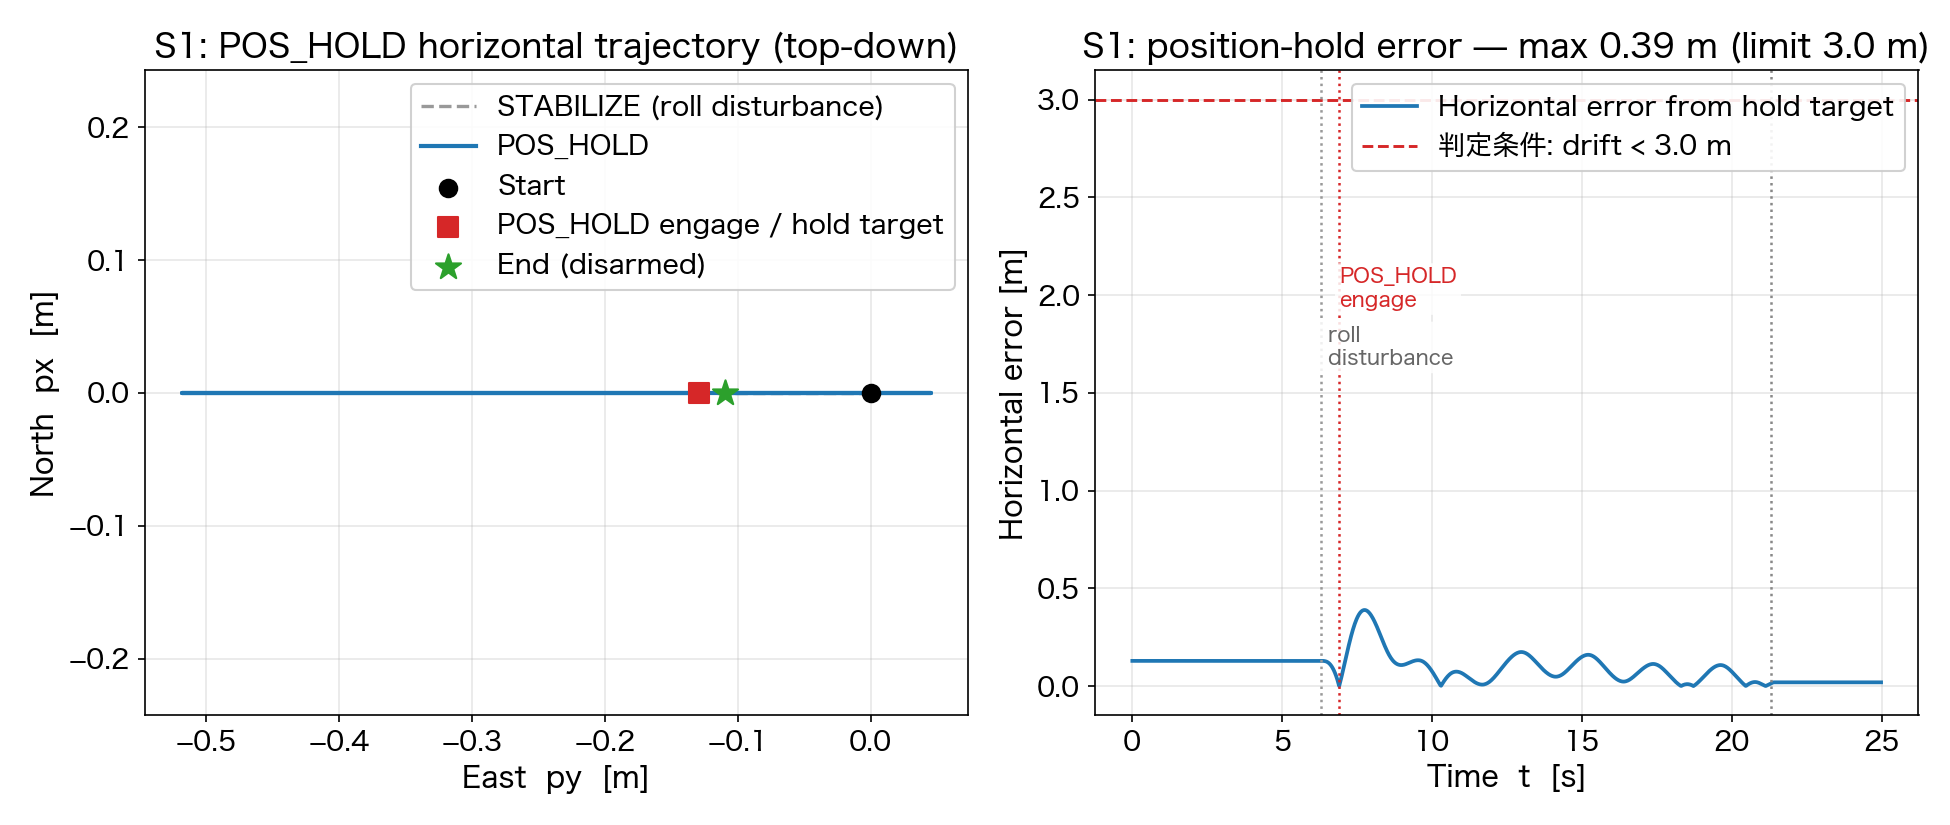
\includegraphics[width=\textwidth, height=0.5\textheight, keepaspectratio]{../fallback/S1_pos_hold_xy.png}

  {\scriptsize \code{pos\_roll.scn}（vehicle）: 離陸 $\to$ ロール外乱 $\to$ POS\_HOLD 係合 $\to$ 保持。係合後の水平ドリフト最大 0.39\,m}
  % Web版のみ: 静止グラフの代わりにPOS_HOLD飛行動画（MuJoCo 3D + 状態グラフ）を見せる
  % @web: video=../fallback/S1_pos_hold_flight.mp4 caption=POS_HOLD 飛行（MuJoCo 3D + 状態グラフ）
  % @web: layout=replace
\end{frame}

% ------------------------------------------------------------------
\begin{frame}{デモ②の期待結果: 高度と姿勢}
  \centering
  \vspace{0.3em}

  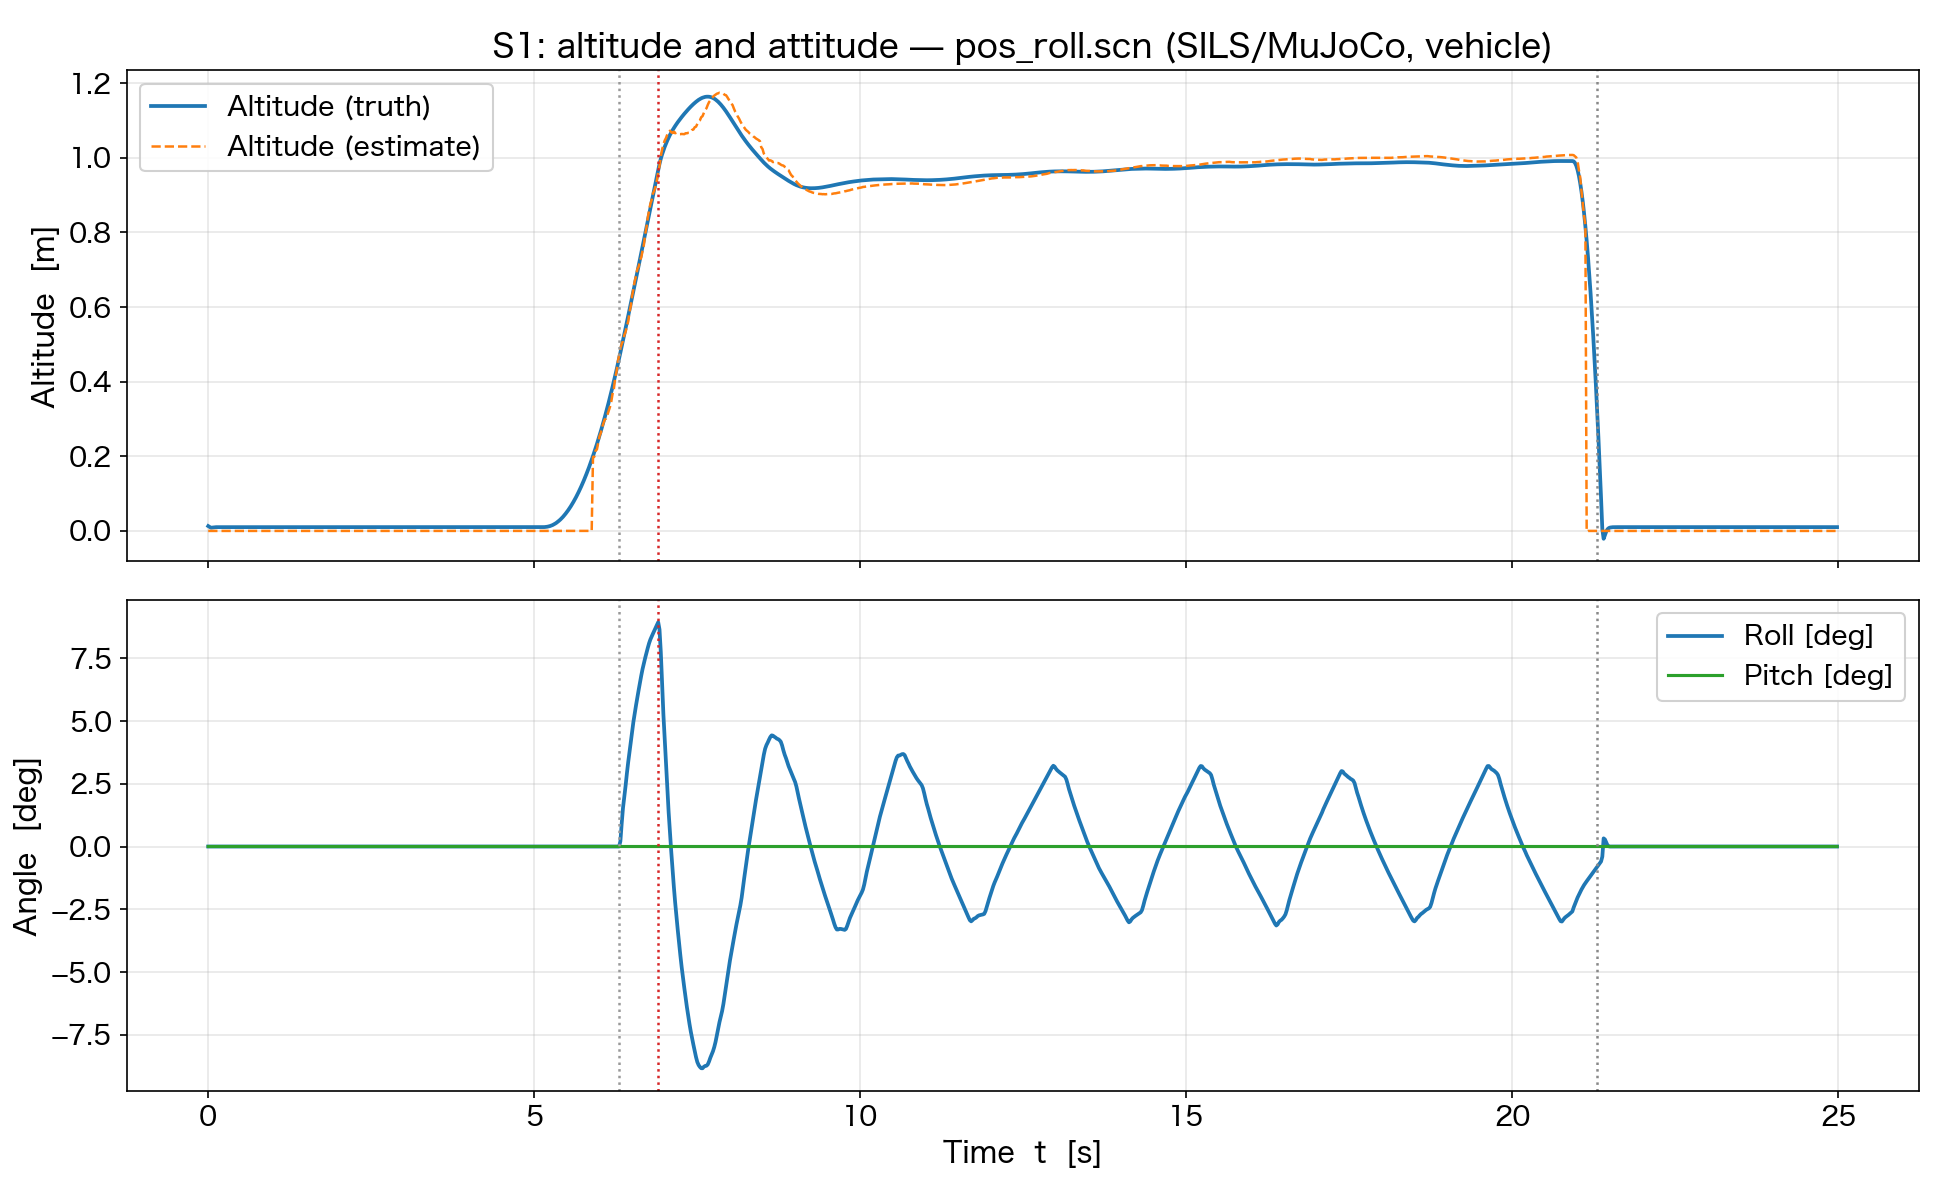
\includegraphics[width=\textwidth, height=0.6\textheight, keepaspectratio]{../fallback/S1_altitude_attitude.png}

  {\scriptsize 同じ飛行の高度と姿勢角の時系列。外乱直後の傾きが位置制御で戻る}
\end{frame}

% ------------------------------------------------------------------
\begin{frame}{復習パス\later}
  \begin{table}
    \centering\footnotesize
    \setlength{\tabcolsep}{4pt}
    \begin{tabular}{>{\raggedright\arraybackslash}p{35mm}>{\raggedright\arraybackslash}p{35mm}>{\raggedright\arraybackslash}p{65mm}}
      \hline
      \textbf{コマンド} & \textbf{対象} & \textbf{文書} \\
      \hline
      \code{sf sim run vpython} & シミュレータ操縦 & \code{docs/\allowbreak architecture/\allowbreak simulation-policy.md} \\
      \code{sf sils gui} & SILS シナリオ実行・可視化 & \code{simulator/\allowbreak sils/\allowbreak gui/\allowbreak README.md} \\
      --- & 4階層アクセス & \code{firmware/\allowbreak vehicle/\allowbreak docs/\allowbreak architecture.md \S2} \\
      \hline
    \end{tabular}
  \end{table}
\end{frame}

% ------------------------------------------------------------------
\begin{frame}{チェックポイント}
  \begin{alertblock}{確認事項}
    \begin{itemize}\small
      \item[$\square$] \textbf{何のために}: 制御なしに飛べない機体で設計の循環を一周する、と説明できる
      \item[$\square$] \textbf{どういう考え方で}: 一つのリポジトリ・4 階層の入口・同じコードとモデル、と説明できる
      \item[$\square$] \textbf{何を提供するか}: 機体・ファーム・3 種類のシミュレータ・sf CLI・教材を挙げ、自分の入る層を 1 つ選べる
    \end{itemize}
  \end{alertblock}

  \vspace{0.5em}

  \begin{block}{次のセッション}
    セッション2: 開発環境のセットアップとセンサデータの取得（11:00 -- 12:00）--- 全体像を見た次は、実際に手を動かしてセンサの値を読む番
  \end{block}
\end{frame}

